% encoding: utf8
% !TEX encoding = utf8
% !TeX spellcheck = pl_PL

\chapter{Podstawy teoretyczne\label{chap:przeglad_literatury}}
Dyskutowane w~pracy algorytmy znane są w~wielu różnych odmianach. Poniżej zaprezentowano wersje używane w~trakcie dalszych badań. 

Do dalszych rozważań możemy zdefiniować uchyb jako:
\begin{equation}
	\boldsymbol{e_x} = \boldsymbol{x_d} - \boldsymbol{x}
\end{equation}
gdzie:
\begin{itemize}
\item $\boldsymbol{x_d}$ to wektor zadanych pozycji uogólnionych
\item $\boldsymbol{x}$ to wektor pozycji uogólnionych
\end{itemize}

\section{Sterowanie impedancyjne}
Prawo sterowania impedancyjnego \cite{bib:impedance}, \cite{wiki:Impedance_control} w~przestrzeni operacyjnej sprawia, że chwytak robota zachowuje się jak przytwierdzony do układu ze sprężyną i~amortyzatorem, gdzie drugi koniec tego układu jest pozycją zadaną. Pojawienie się nieprzewidzianych sił zewnętrznych powoduje, że uchyb pozycji nie jest minimalizowany za wszelką cenę. Przy kontakcie z~otoczeniem stawy robota są w~pewnym stopniu sprężyste i~miękkie. W~konsekwencji robot ugina się przed otaczającym go środowiskiem. Ma to zazwyczaj miejsce w~chwili zderzenia z~nieprzewidzianą przeszkodą. 

\subsection{Przypadek prosty}
W najprostszym przypadku możemy więc opisać takie prawo jako układ: 

	\begin{equation}
	F = kx + d\dot{x} + F_{ext}
	\end{equation}

gdzie:
\begin{itemize}
\item $F$ to siła wynikowa
\item $k$ to parametr sztywności
\item $d$ to parametr tłumienia
\item $F_{ext}$ to nieznana siła zewnętrzna działająca na układ
\end{itemize} 

\subsection{Prawo sterowania}
\label{sec:impedancyjne}

Prawo sterowania można sformułować  jako wektor siły uogólnionej:
\begin{equation}
\boldsymbol{\mathcal{F}} = \boldsymbol{K_x}\boldsymbol{e_x} + \boldsymbol{D_x}\dot{\boldsymbol{e_x}}
\end{equation}

gdzie:
\begin{itemize}
\item $\boldsymbol{K_x}$ to diagonalna macierz sprężystości
\item $\boldsymbol{D_x}$ to diagonalna macierz tłumienia
\item $\boldsymbol{\mathcal{F}_{ext}}$ to wektor nieznanych uogólnionych sił zewnętrznych
\end{itemize}

\subsection{Sterowanie w~przestrzeni konfiguracyjnej}
\label{chap:jakobian}
W rzeczywistym ramieniu robotycznym zadajemy momenty na poszczególne stawy robota. Opisane w~podrozdziale \ref{sec:impedancyjne} prawo sterowania opisuje przestrzeń operacyjną $\boldsymbol{\mathcal{F}}$.  Wartości wektora momentów $\boldsymbol{\tau}$ można uzyskać z~jakobianu $\boldsymbol{J}$:

\begin{equation}
\boldsymbol{\tau} = \boldsymbol{J}^T(\boldsymbol{q})\boldsymbol{\mathcal{F}}
\end{equation}

\section{Sterowanie PID}
\label{chap:key}
Regulator PID (ang. Proportional Integral Derivative) \cite{bib:pidTito}, \cite{bib:pidMimo} jest popularnym prawem sterowania automatycznego. Podstawowym celem algorytmu jest minimalizacja uchybu. Uchyb statyczny jest minimalizowany za wszelką cenę nawet jeśli miałoby to spowodować uszkodzenia. Uchyby dynamiczne nie są już tak dobrze kompensowane.

Człon proporcjonalny algorytmu pozwala na wzmocnienie uchybu i~w~ten sposób odjęcie go od sygnału sterującego. Człon całkujący algorytmu sumuje przeszłe błędy i~odejmuje od sterowania ich sumę. Człon różniczkujący wzmacnia sygnał sterujący, gdy wartość błędu zmienia się w~celu przyspieszenia regulacji.
\subsection{Przypadek prosty}
W jednowymiarowym przypadku prawo sterowania ma postać:
\begin{equation}
F = Pe + I\int_{0}^{t}e dt + D\frac{de}{dt}
\end{equation}

gdzie:
\begin{itemize}
	\item $e$ to uchyb
	\item $P$ to parametr członu proporcjonalnego
	\item $I$ to parametr członu całkującego
	\item $D$ to parametr członu różniczkującego
\end{itemize}


\subsection{Przypadek wielowymiarowy}
Rozpatrując wektor siły uogólnionej możemy założyć w~uproszczeniu, że prawo sterowania rozpatruje każdą z~wartości wektora niezależnie. Prawo sterowania można zapisać w~postaci:
\begin{equation}
\boldsymbol{\mathcal{F}} = \boldsymbol{P}\boldsymbol{e_x} +\int_{0}^{t}  \boldsymbol{I}\boldsymbol{e_x}dt + \boldsymbol{D}\dot{\boldsymbol{e_x}}
\end{equation}
gdzie:
\begin{itemize}
	\item $\boldsymbol{P_x}$ to diagonalna macierz proporcjonalności
	\item $\boldsymbol{I_x}$ to diagonalna macierz członu całkowania
	\item $\boldsymbol{D_x}$ to diagonalna macierz członu różniczkującego
\end{itemize}

\section{Estymacja siły uogólnionej w~końcówce}
\label{chap:estymacja}
Dla ramienia robotycznego możemy opisać siły występujące w~samym ramieniu zgodnie ze wzorem:
\begin{equation}
\boldsymbol{\mathcal{F}_m} = \boldsymbol{\mathcal{F}_m}(\boldsymbol{x}, \dot{\boldsymbol{x}}, \ddot{\boldsymbol{x}}, \boldsymbol{q}, \dot{\boldsymbol{q}}) = \boldsymbol{\Lambda}(\boldsymbol{q})\boldsymbol{\ddot{x}} + \boldsymbol{\mu}(\boldsymbol{x}, \boldsymbol{\dot{x}}) + \boldsymbol{\gamma}(\boldsymbol{q}) + \boldsymbol{\eta}(\boldsymbol{q}, \boldsymbol{\dot{q}}) + \boldsymbol{\mathcal{F}_{ext}}
\label{eq:ramie}
\end{equation}

gdzie:
\begin{itemize}
	\item $\boldsymbol{\mathcal{F}}$ to wektor sił wynikowych
	\item $\boldsymbol{\Lambda}$ to dodatnio określona macierz inercji w~przestrzeni zadań
	\item $\boldsymbol{\mu}$ to macierz sił Coriolisa i~sił odśrodkowych	
	\item $\boldsymbol{\gamma}$ to wektor sił grawitacji
	\item $\boldsymbol{\eta}$ to macierz sił tarcia oraz nieuwzględnionych sił
	\item $\boldsymbol{q}$ to wektor położeń stawów w~przestrzeni konfiguracyjnej
	\item $\boldsymbol{x}$ to wektor położeń końcówki w~przestrzeni zadań
	\item $ \boldsymbol{\mathcal{F}_{ext}}$ to nieznany wektor sił zewnętrznych działających na układ
\end{itemize} 

Przy wyliczaniu i estymowaniu sił działających na końcówkę należy pamiętać, że w~końcówce występują siły wygenerowane przez prawo sterowania oraz rzeczywiste siły występujące w~układzie. Wzór estymujący rzeczywistą wartość siły uogólnionej w~końcówce można zapisać jako:
\begin{equation}
\boldsymbol{\mathcal{\hat{F}}} = \boldsymbol{\mathcal{F}} + \boldsymbol{\mathcal{F}_m}(\boldsymbol{x}, \dot{\boldsymbol{x}}, \ddot{\boldsymbol{x}}, \boldsymbol{q}, \dot{\boldsymbol{q}})
\end{equation}

gdzie $\boldsymbol{\mathcal{F}}$ to wektor sił uogólnionych wyliczony prawem sterowania.

% \section{Ocena jakości algorytmów sterowania}
\section{Jakość sterowania}
\label{chap:ape}
Prostym sposobem oceny jakości algorytmu sterowania jest konfrontacja rzeczywistych pozycji ramienia robota z~zadanymi. W~pracy przyjęto metrykę APE (ang. Absolute Trajectory Error) \cite{bib:ape}. Metryka jest popularnym wskaźnikiem testowania algorytmów SLAM (ang. Simultaneous Localization and Mapping), ale może być też użyta do porównania trajektorii zadanej przez interpolator  oraz osiągniętej w~rzeczywistości (rys. \ref{fig:przykl_ape}). 

Dwie trajektorie są opisane w~postaci list wektorów sił uogólnionych $\boldsymbol{P}_{1..n}$ oraz $\boldsymbol{Q}_{1..n}$ gdzie $n$ to ilość próbek. Dla każdej chwili czasowej $i$ jest wyliczany błąd postaci:
\begin{equation}
\boldsymbol{E}_i = \boldsymbol{Q}_i^{-1}\boldsymbol{S}\boldsymbol{P}_i
\end{equation}
Macierz $\boldsymbol{S}$ jest optymalnym, w~sensie metody najmniejszych kwadratów, rzutowaniem wektora $\boldsymbol{Q}_i$ na wektor $\boldsymbol{P}_i$ - znalezionym za pomocą metody Horna \cite{bib:horn}. 

Błąd całkowity jest wyliczany jako błąd średnio-kwadratowy:
\begin{equation}
RMSE(\boldsymbol{E}_{1..n}) = \sqrt{\frac{1}{n}\sum_{i=1}^{n}||\boldsymbol{E}_i||^2}
\end{equation}.



\begin{figure}
	\centering
		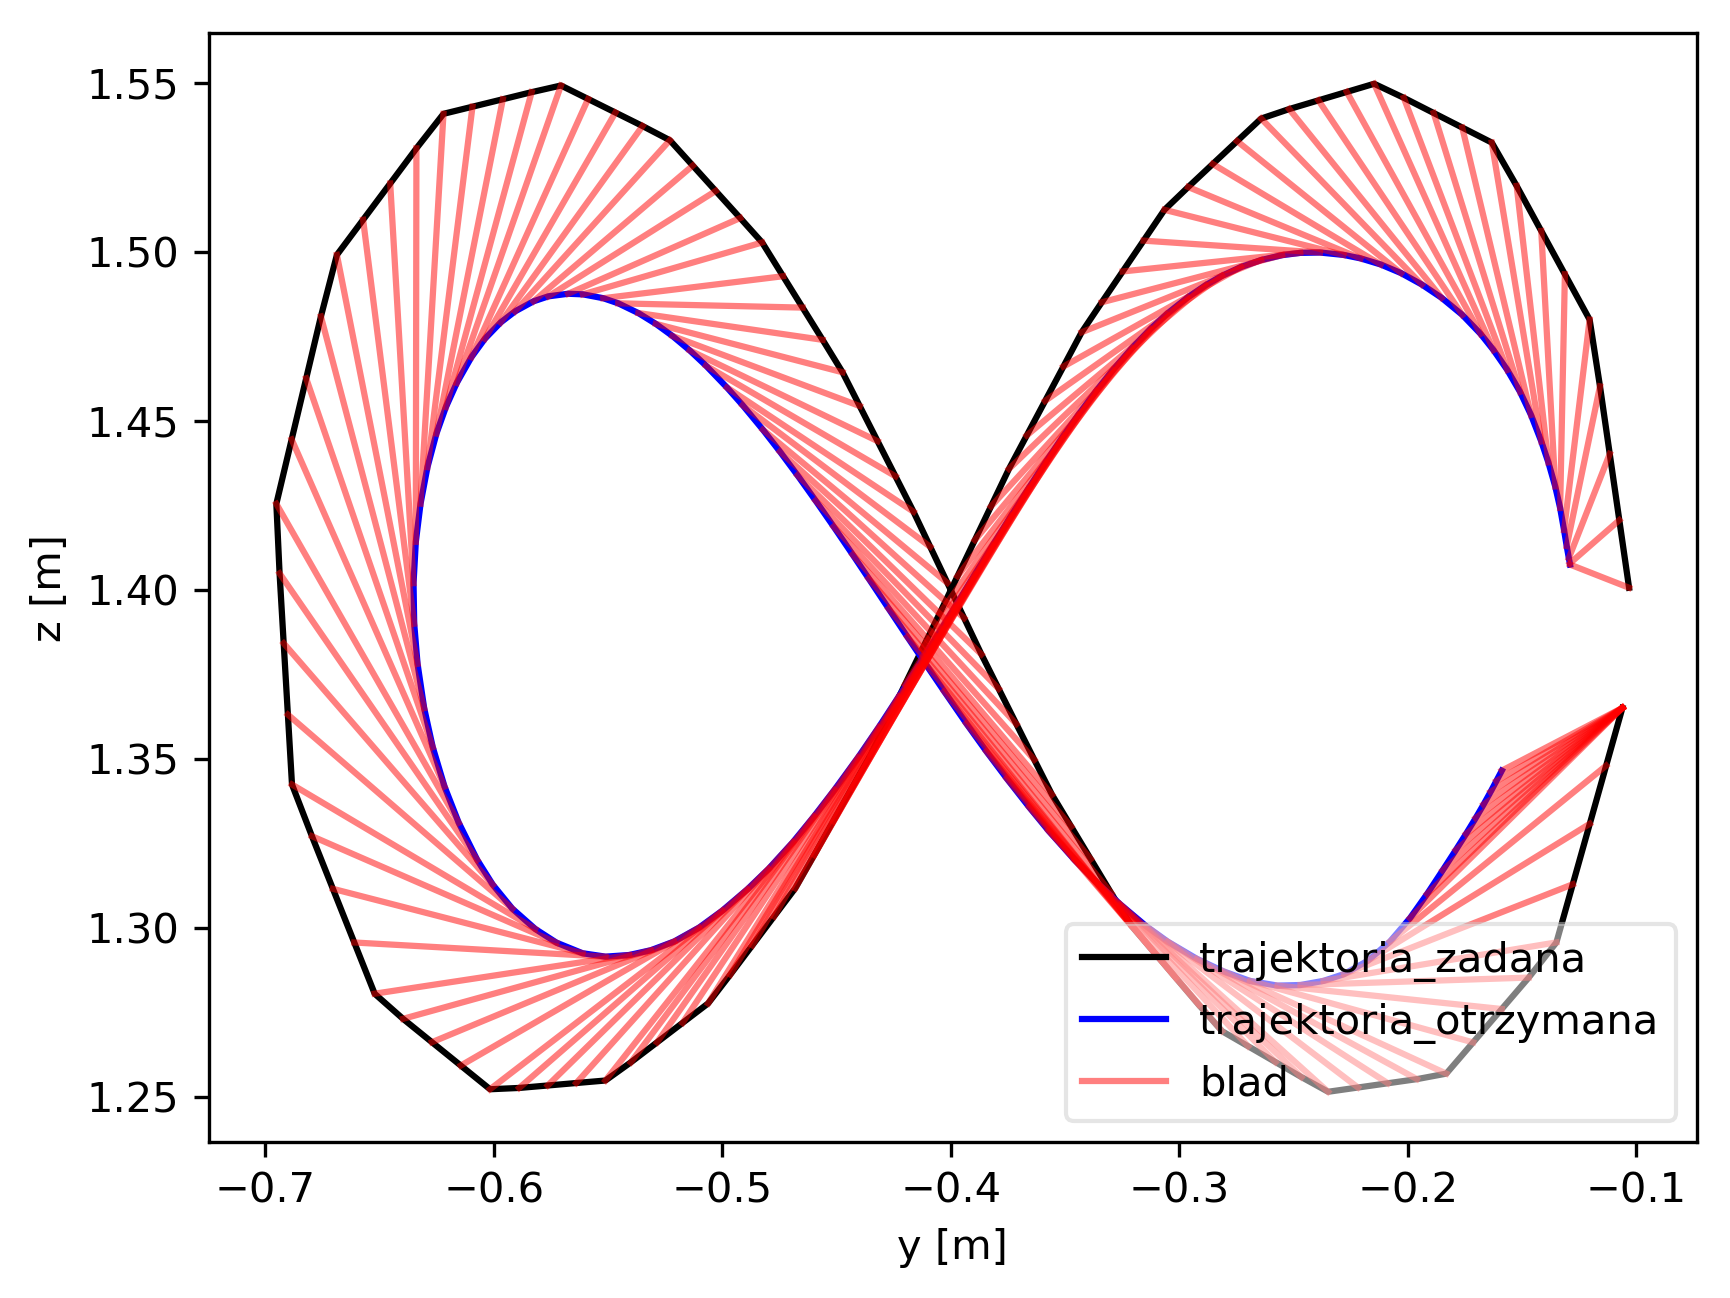
\includegraphics[width=.45\textwidth]{./velma/przerobione_testy/out/osemka/yz_ate_plot_podnoszenie_miekki_bez_brak.png}
		\caption{Rysunek przedstawia rzut APE w~dwóch wymiarach. Czarną i~niebieską linią oznaczono zadaną i osiąganą trajektorię. Linie czerwone łączą odpowiednie punkty na obydwu trajektoriach i~obrazują błąd pomiędzy nimi.}
		\label{fig:przykl_ape}
\end{figure}

% \subsection{Jakość kontaktu z~otoczeniem \label{chap:ocenakonaktu}}

% Największą zaletą sterowania impedancyjnego jest ugięcie ramienia robota w~momencie kolizji ze środowiskiem. Ocena jakości tej cechy może być opisana jako odchylenie pozycji stawów $\boldsymbol{q}_i$ w~stosunku do ustalonej pozycji sprzed kolizji $\boldsymbol{q}$ w~chwili $i$.


\section{Teoria agenta upostaciowionego}
Agentem możemy nazwać jednostkę, która jest: zdolna do komunikowania się ze środowiskiem, zdolna do monitorowania swego otoczenia i~podejmowania autonomicznych decyzji. Taka definicja gwarantuje spełnienie wielu cech, których oczekujemy od nowoczesnych systemów robotycznych. Z~definicji agenty są w~stanie samodzielnie reagować na zmiany zachodzące w~środowisku w~sposób inteligentny. Rozszerzeniem teorii agentowej jest teoria agenta upostaciowionego \cite{bib:agent1} \cite{bib:agent2}. Agent upostaciowiony cechuje się tym czym zwykły agent oraz posiada fizyczne ciało. Agenty oraz podsystemy mogą komunikować się poprzez bufory.


W teorii agenta upostaciowionego występują pojęcia rzeczywistych efektorów i~receptorów. Służą one odpowiednio do oddziaływania na środowisko i~do pozyskiwania wiedzy o~tym środowisku. W~praktyce oznacza to, że rzeczywistym efektorem może być silnik a~rzeczywistym receptorem enkoder. 

Agent upostaciowiony $a$  (rys. \ref{fig:upostaciowiony}) może się składać z~trzech podsystemów:
\begin{itemize}
	\item Podsystemu sterowania $c$ który zajmuje się podejmowaniem decyzji na podstawie danych z~innych podsystemów. Agent może mieć tylko jeden podsystem sterowania.
	\item Wirtualnego efektora $e$ który pośredniczy w~komunikacji pomiędzy podsystemem sterowania i~rzeczywistym efektorem.
	\item Wirtualnego receptora $r$ który pośredniczy w~komunikacji pomiędzy podsystemem sterowania i~rzeczywistym receptorem.
\end{itemize}

W podejściu komponentowym wspomnianej teorii podsystemy składają się z~komponentów, czyli algorytmów. Każdy z~podsystemów może mieć wiele komponentów. Podsystem posiada zdefiniowaną maszynę stanów. Stany maszyny mogą się zmieniać przy pomocy funkcji przejścia (predykatów). Stan maszyny definiuje tak zwane zachowanie podsystemu, czyli sposób reakcji poprzez uruchomienie konkretnych komponentów. 

\begin{figure}
	\centering
	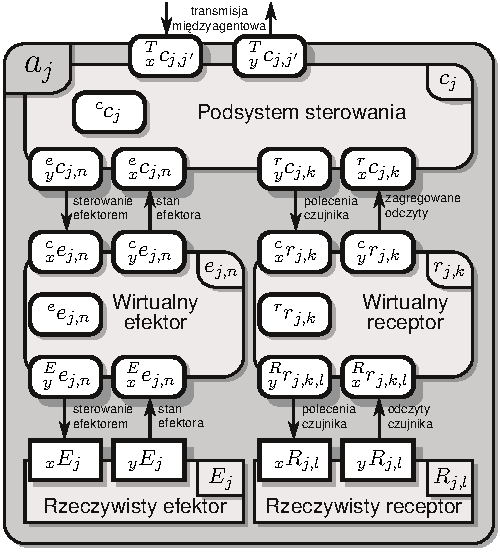
\includegraphics[width=.6\textwidth]{images/agent_structure.pdf}
	\caption{Rysunek przedstawia schemat budowy agenta upostaciowionego \cite{Zielinski:2014_kkr_relacje-twiki}. Typ podsystemu oznaczany jest dużą literą. Podsystemy i~bufory posiadają prawy dolny indeks. Typ podsystemu jest oznaczany lewym dolnym indeksem.  Typ buforu jest oznaczany lewym dolnym indeksem ($x$ - wejściowy, $y$ - wyjściowy).}
	\label{fig:upostaciowiony}
\end{figure}